\documentclass[../main.tex]{subfiles}

%\graphicspath{{\subfix{../images/}}}

\begin{document}

\section{{\sc Ryden} - Introduction to Cosmology, 2016}
\subsection{Exercise 2.1}
The power emitted by a surface $dA$ under the angle $\theta$ ($\theta=0$ is perpendicular to the surface $dA$) into the solid angle $d\Omega$ is $B_\nu\cos\theta\,dA\,d\Omega\,d\nu$ with
\begin{align}
B_\nu(\nu,T)=\frac{2h\nu^3}{c^2}\frac{1}{e^{h\nu/kT}-1}
\end{align}
this is related to the spectral energy density (eqn 2.27) of the photon field by
\begin{align}
\varepsilon(\nu)=u_\nu=\frac{4\pi}{c}B_\nu.
\end{align}
The angular integration (for $dA$ in the $xy$ plane) gives
\begin{align}
\int\cos\theta\,d\Omega=\int_0^{2\pi}\int_0^{\pi/2}\cos\theta\,\sin\theta\;d\theta\,d\phi
\end{align}
and therefore with $\rho=m/V$ and $V=4/3\pi R^3$ we obtain
\begin{align}
P&=\int B_\nu\cos\theta\,dA\,d\Omega\,d\nu\\
&=\pi\int B_\nu\,dA\,d\nu\\
&=\frac{2\pi^5k^4}{15c^2h^3}T^4\int dA\\
&=\frac{2\pi^5k^4}{15c^2h^3}T^4\cdot 4\pi R^2\\
&=\frac{2\pi^5k^4}{15c^2h^3}T^4\cdot \left(\frac{6\sqrt{\pi}m}{\rho}\right)^{2/3}
\end{align}
which gives for $m=75$kg a power of 440W. The net power is obviously smaller $P_\text{net}=\sigma A(T_\text{body}^4-T_\text{ambient}^4)$. 

\subsection{Exercise 2.2}
The photon number density is given by (eqn 2.30)
\begin{align}
n(\nu)=\frac{\varepsilon(\nu)}{h\nu}=\frac{8\pi\nu^2}{c^3}\frac{1}{e^{h\nu/kT}-1}
\end{align}
then the flux across the projected surface of the sphere $\pi R^2$ from each direction is given by  
\begin{align}
N&=\int d\Omega\int d\nu\,\pi R^2 cn(\nu)\\
&=4\pi^2 cR^2\int d\nu\, n(\nu)\\
&=\zeta(3)\frac{64\pi^3R^2}{c^2h^3}(kT)^3\\
&=3.2\cdot10^{17}
\end{align}
assuming $m=\rho V=75$kg. Analog
\begin{align}
P&=\int d\Omega\int d\nu\,\pi R^2 c\varepsilon(\nu)\\
&=4\pi^2 cR^2\int d\nu\, varepsilon(\nu)\\
&=\frac{32\pi^7R^2}{15c^2h^3}(kT)^4\\
&=3.3\cdot10^{-5}\text{W}
\end{align}

\subsection{Exercise 2.3}
Combining the results
\begin{align}
P_\text{rad}&=-440\text{W}\\
P_\text{absCMB}&=3.3\cdot10^{-5}\text{W}\\
P_\text{tot}&=-440W
\end{align}
So the astronaut is loosing heat and can not overheat.
The astronauts energy loss is given by
\begin{align}
\Delta E_\text{heat}=mC\Delta T\equiv P_\text{tot}\Delta t\\
\rightarrow \frac{\Delta t}{\Delta T}=\frac{mC}{P_\text{tot}}=716\text{s/K}=12\text{min/K}
\end{align}
therefore so the lack of oxygen seems to be most likely.

\subsection{Exercise 2.4}
\begin{align}
z(r)&=\frac{\lambda(r)-\lambda_\text{em}}{\lambda_\text{em}}\quad\rightarrow\quad\lambda(r)=[1+z(r)]\lambda_\text{em}\\
E(r)&=hc\frac{1}{\lambda(r)}=\frac{hc}{[1+z(r)]\lambda_\text{em}}\\
\frac{dE}{dr}&=-kE\quad\rightarrow\quad z'-k(1+z)=0\\
&\quad\rightarrow\quad z(r)=ce^{kr}-1 \quad(z(0)=0) \\
&\quad\rightarrow\quad z(r)=e^{kr}-1\\
&\quad\rightarrow\quad z(r)\approx kr
\end{align}
with $k=H_0/c$

\subsection{Exercise 2.5}
With
\begin{align}
n(\nu)&=\frac{\varepsilon(\nu)}{h\nu}=\frac{8\pi\nu^2}{c^3}\frac{1}{e^{h\nu/kT}-1}\\
n_\gamma=&\int d\nu\,n(\nu)\\
&=\frac{16\zeta(3)\pi}{c^3h^3}(kT)^3
=\frac{2\zeta(3)}{\pi^2c^3\hbar^3}(kT)^3
\end{align}
then
\begin{align}
n(h\nu>E_0)&=\frac{8\pi}{c^3}\int_{E_0/h}^\infty\frac{\nu^2}{e^{h\nu/kT}-1}d\nu\\
&\overset{h\nu>E_0\gg kT}{\simeq}\frac{8\pi}{c^3}\int_{E_0/h}^\infty e^{-h\nu/kT}\nu^2 d\nu\\
&=\frac{8\pi kT}{c^3h^3}e^{-E_0/kT}(E_0^2+2E_0kT+2(kT)^2)\\
&\simeq\frac{8\pi kT}{c^3h^3}e^{-E_0/kT}E_0^2
\end{align}
then
\begin{align}
\frac{n(h\nu>E_0)}{n_\gamma}=\frac{1}{2\zeta(3)}e^{-E_0/kT}\left(\frac{E_0^2}{kT}\right)^2
\end{align}
Using this result we obtain $5.8\%$ of infrared photons. Exact numerical integration gives $6\cdot10^{-4}\%$ radio waves (or longer), $91.6\%$ microwaves, $8.4\%$ infrared, $0\%$ optical (and shorter).

\subsection{Exercise 2.6}
Now
\begin{align}
n(h\nu<E_0)&=\frac{8\pi}{c^3}\int_0^{E_0/h}\frac{\nu^2}{e^{h\nu/kT}-1}d\nu\\
&\overset{h\nu<E_0\ll kT}{\simeq}\frac{8\pi}{c^3}\int_{E_0/h}^\infty \frac{kT}{h\nu}\nu^2d\nu\\
&=\frac{4E_0^2 \pi kT}{c^3h^3}
\end{align}
then
\begin{align}
\frac{n(h\nu<E_0)}{n_\gamma}=\frac{E_0^2}{4\zeta(3)k^2T^2}
\end{align}
For $\lambda>3$cm ($hc/\lambda=h\nu<E_0=hc/\lambda_0$) we obtain $0.6\%$.


\subsection{Exercise 3.2}
We replace $d\theta$ by $d\varphi$! Calculating the size of the object as distance on the sphere of radius $R$
\begin{align}
dl^2
&=R^2(d\theta^2+\sin^2\theta d\varphi^2)\\
&=R^2\sin^2\theta d\varphi^2
\end{align}
with $\theta=r/R$. Then
\begin{align}
dl&=R\sin\frac{r}{R} \cdot d\varphi\\
&\rightarrow d\varphi=\frac{dl}{R\sin\frac{r}{R}}
\end{align}
For $r\rightarrow\pi R$ $d\varphi$ increases to $2\pi$
\begin{figure}[!h]
\centering
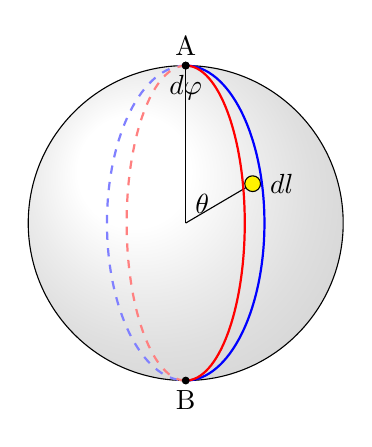
\begin{tikzpicture}
  \shade[ball color=white,opacity=0.25](3,3)circle (2);
  \draw(3,5) -- (3,3)node[above right]{$\theta$};
  \draw(3,3) -- (3.85,3.5);
  \draw(3,3)circle(2);
  \draw[black,fill=yellow](3.85,3.5)circle(0.1)node[right]{$\;dl$};
  \draw[thick,blue](3,5)arc(90:-90:1cm and 2cm);
  \draw[thick,blue!50,dashed](3,5)arc(90:-90:-1cm and 2cm);
  \draw[thick,red](3,5)arc(90:-90:0.75cm and 2cm);
  \draw[thick,red!50,dashed](3,5)arc(90:-90:-0.75cm and 2cm);
  \fill(3,5)circle(0.05)node[above]{A};
  \fill(3,5)circle(0.05)node[below]{$d\varphi$};
  \fill(3,1)circle(0.05)node[below]{B};
\end{tikzpicture}
\begin{tikzpicture}
\draw[white](0,0) -- (1,0);
\end{tikzpicture}
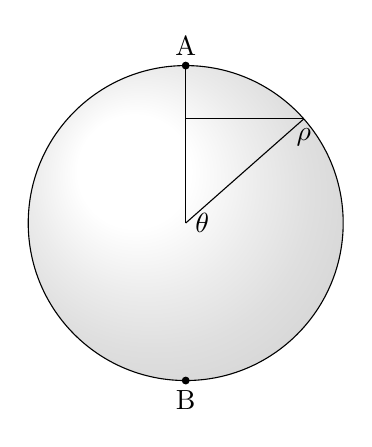
\begin{tikzpicture}
  \shade[ball color=white,opacity=0.25](3,3)circle (2);
  \draw(3,5) -- (3,3)node[right]{$\theta$};
  \draw(3,3) -- (4.5,4.323);
  \draw(3,4.323) -- (4.5,4.323)node[below]{$\rho$};
  \draw(3,3)circle(2);
  \fill(3,5)circle(0.05)node[above]{A};
  \fill(3,1)circle(0.05)node[below]{B};
\end{tikzpicture}
\caption{(left) Ex 3.2. Spherical universe, Observer at A, object of size $dl$ at distance $r$, (right) Ex 3.3. Spherical universe, Observer at A}
\end{figure}

\subsection{Exercise 3.3}
Simple geometry
\begin{align}
\theta&=2\pi\frac{r}{2\pi R}=\frac{r}{R}\\
\sin\theta&=\frac{\rho}{R}\\
C=2\pi\rho
\end{align}
gives
\begin{align}
C&=2\pi\rho\\
&=2\pi R \sin\theta\\
&=2\pi R \sin\frac{r}{R}.
\end{align}
For the euclidean case we get of course $C_\text{Euclid}=2\pi r$. Then
\begin{align}
\Delta s &= C_\text{Euclid}-C\\
&=2\pi (r-R \sin\frac{r}{R})\\
&\simeq\frac{\pi r^3}{3R^2}-\frac{\pi r^5}{60R^2}\\
&\simeq33.8\text{ km}
\end{align}

\subsection{Exercise 3.4}
\begin{enumerate}
\item $\kappa=+1$
With
\begin{align}
\alpha+\beta+\gamma=\frac{A}{R^2}+\pi
\end{align}
we see that each angle can be maximally $\pi$. So
\begin{align}
A_{\max}=(3\pi-\pi)R^2=2\pi R^2.
\end{align}
It is easy to see that such a (degenerated) triangle (half sphere) can be realized. 

A bit more formal - integrating over a triangle-shape slice
\begin{align}
A&=\int_0^\alpha\int_0^\alpha R^2\sin\theta\,d\theta\,d\phi\\
&=R^2(\alpha-\alpha\cos\alpha)\\
A_\text{max}&=A(\alpha=\pi)=2\pi R^2
\end{align}

\item $\kappa=0$
There is no limited to the triangle size.


\item $\kappa=-1$
With
\begin{align}
A=(\pi-\alpha-\beta-\gamma)R^2
\end{align}
we see that the potential maximum is $A_\text{max}=\pi R^2$. Now we need to show that such a triangle exists.

\end{enumerate}

\subsection{Exercise 3.5}
With
\begin{align}
dx&=\frac{x}{r}dr+\frac{x}{\sin\theta}\cos\theta\,d\theta+\frac{x}{\cos\phi}(-\sin\phi)\,d\phi\\
dy&=\frac{y}{r}dr+\frac{y}{\sin\theta}\cos\theta\,d\theta+\frac{y}{\sin\phi}\cos\phi\,d\phi\\
dz&=\frac{z}{r}dr+\frac{z}{\cos\theta}(-\sin\theta)d\theta
\end{align}
we obtain
\begin{align}
ds^2&=dx^2+dy^2+dz^2\\
&=dr^2+r^2(d\theta^2+\sin^2\theta d\phi^2)
\end{align}

\subsection{Exercise 4.1}
\begin{align}
E_\text{sun}&=M_\text{sun}c^2=1.79\cdot10^{47}\text{J}\\
E_\Lambda&=\varepsilon_\Lambda\frac{4}{3}\pi R^3=1.1\cdot10^{25}\text{J}
\end{align}



\section{{\sc Boerner} - The Early Universe - Facts and Fiction (4th edition)}
\subsection{1.1 Friedman equations}
\begin{enumerate}
\item The Friedman equations in book contain a small typo ($\rho=\varrho$)
\begin{align}
    (A)\qquad \ddot R&=-\frac{4\pi}{3}(\varrho+3p)GR+\frac{1}{3}\Lambda R\\
    (B)\qquad  \dot R^2&=\frac{8\pi}{3}G\varrho R^2+\frac{1}{3}\Lambda R^2-K\\
    (C)\qquad 0&=(\varrho R^3)^\cdot+p(R^3)^\cdot
\end{align}
Calculating the time derivative of (B)
\begin{align}
    2\dot{R}\ddot{R}&=\frac{8\pi}{3}G(\dot{\varrho}R^2+2\varrho R\dot{R})+\frac{2}{3}\Lambda R\dot{R}\\
    \ddot{R}&=\frac{R}{3}\left(4\pi G\dot\varrho \frac{R}{\dot{R}}+8\pi G\varrho +\Lambda\right)
\end{align}
and simplifying (A)
\begin{align}
    \ddot R&=\frac{R}{3}\left(-4\pi G(\varrho+3p)+\Lambda\right)
\end{align}
Combining both yields
\begin{align}
    \dot\varrho \frac{R}{\dot{R}}+2\varrho=-(\varrho+3p)\\
    \dot\varrho R=-3(\varrho+p)\dot{R}
\end{align}
which is (C). Rearranging the order of the steps gives the other two  cases.
\item From (C) we have
\begin{align}
    \dot\varrho &=-3(\varrho+p)\frac{\dot{R}}{R}\\
    &=-3\varrho\left(1+k\varrho^{\gamma-1}\right)\frac{\dot{R}}{R}
\end{align}
which can be rearranged and integrated
\begin{align}
    \frac{\dot{R}}{R}&=\frac{\dot\varrho}{-3\varrho\left(1+k\varrho^{\gamma-1}\right)}\\
    &\rightarrow-\frac{1}{3(1-\gamma)}\log(k+\varrho^{1-\gamma})=\log R+c\\
    &\rightarrow\log(k+\varrho^{1-\gamma})=-3(1-\gamma)\log R+c'\\
    &\rightarrow k+\varrho^{1-\gamma}=e^{-3(1-\gamma)\log R+c'}\\
    &\rightarrow k+\varrho^{1-\gamma}=c''R^{-3(1-\gamma)}\\
    &\rightarrow \varrho=\left(c''R^{3(\gamma-1)}-k\right)^{1/(1-\gamma)}
\end{align}
with
\begin{align}
    c''&=\frac{k+\varrho_0^{1-\gamma}}{R_0^{3(\gamma-1)}}\\
    &\quad\rightarrow\quad\varrho=\left([k+\varrho_0^{1-\gamma}]\frac{R}{R_0}^{3(\gamma-1)}-k\right)^{1/(1-\gamma)}\\
    &\quad\rightarrow\quad\varrho=\left(k\left[\frac{R}{R_0}^{3(\gamma-1)}-1\right]+\left[\frac{R^3}{\varrho_0R_0^3}\right]^{\gamma-1}\right)^{1/(1-\gamma)}
\end{align}

We obtain from (B)
\begin{align}
    \dot R^2-\left(\frac{8\pi}{3}G\varrho +\frac{1}{3}\Lambda\right) R^2=-K
\end{align}
which we can interpret as motion of a particle in a changing $-R^2$ potential.

\begin{center}
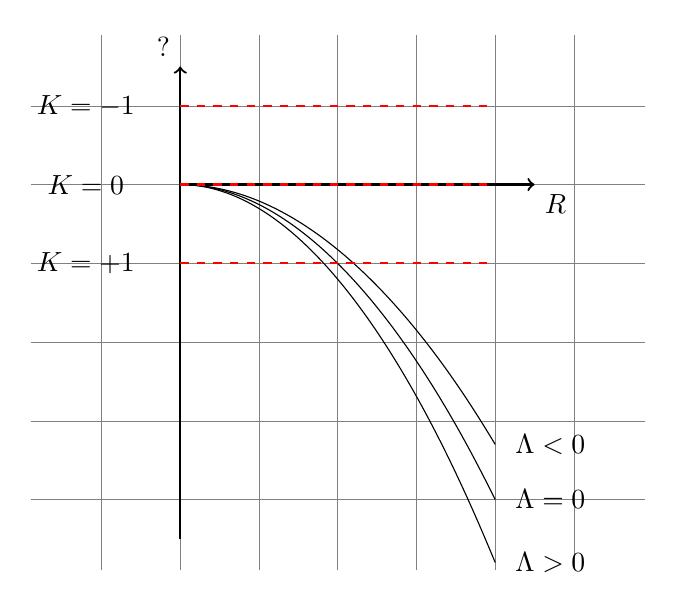
\begin{tikzpicture}
\draw[step=1cm,gray,very thin] (-1.9,-4.9) grid (5.9,1.9);
\draw[thick,->] (0,0) -- (4.5,0) node[anchor=north west] {$R$};
\draw[thick,->] (0,-4.5) -- (0,1.5) node[anchor=south east] {?};
\draw (0,0) parabola (4,-4);
\draw (0,0) parabola (4,-3.3);
\draw (0,0) parabola (4,-4.8);

\draw[red,thick,dashed] (0,1) -- (4,1);
\draw[red,thick,dashed] (0,0) -- (4,0);
\draw[red,thick,dashed] (0,-1) -- (4,-1);

\coordinate (A) at (0,1);
\coordinate (B) at (0,0);
\coordinate (C) at (0,-1);
\node[xshift=-1.2cm] at (A) {$K=-1$};
\node[xshift=-1.2cm] at (B) {$K=0$};
\node[xshift=-1.2cm] at (C) {$K=+1$};

\coordinate (AA) at (4,-3.3);
\coordinate (BB) at (4,-4);
\coordinate (CC) at (4,-4.8);
\node[xshift=0.7cm] at (AA) {$\Lambda<0$};
\node[xshift=0.7cm] at (BB) {$\Lambda=0$};
\node[xshift=0.7cm] at (CC) {$\Lambda>0$};
\end{tikzpicture}
\end{center}

\end{enumerate}

\section{{\sc Baumann} - Cosmology (1nd edition)}
\subsection{Problem 1.1 Length scales}
\begin{tabular}{lcc}
\hline 
object & size & size in m \\ 
\hline \hline 
pepper corn & 5mm & 0.005m \\
basketball size 7 (75 cm circumference) & 24cm & 0.24m \\ 
basketball court & 30.62yds & 28m \\ 
\hline 
\end{tabular} 

\begin{enumerate}
\item $R_\text{Moon}$ = 6.5cm, $d_\text{ME}$=11.3m
\item $R_\text{Sun}$ = 55cm, $r_\text{Earth orbit}$=118m, $r_\text{Neptune orbit}$=3544m
\item $d_\text{Solar system}$=0.2mm
\item $R_\text{Solar neigh}$ = 18mm
\item $R_\text{Galaxy}$ = 28cm
\item $R_\text{Local Group}$ = 56cm
\item $R_\text{Super Cluster}$ = 30cm
\end{enumerate} 

\subsection{Problem 1.2 Hubble constant}
\begin{enumerate}
\item $t_{H_0}=14\cdot10^{9}$a
\item $d_{H_0}=140\cdot10^{9}$ly
\item $\rho_0=9\cdot10^{-27}$kg/m$^3$
\item $n_\text{H universe}=\frac{\rho_0 d^3}{m_\text{H}}=10^{79}$, $n_\text{H brain}=\frac{m_\text{brain}}{m_{H_2O}}=10^{26}$
\end{enumerate}

\subsection{Exercise 2.1}
Using the Euler Lagrange equations we obtain
\begin{align}
\frac{\partial L}{\partial r}=mr\dot\phi^2,\quad\frac{\partial L}{\partial\dot r}=mr\dot r\quad&\rightarrow\quad\ddot r=r\dot\phi^2\\
\frac{\partial L}{\partial \phi}=0,\quad\frac{\partial L}{\partial\dot\phi}=mr^2\dot \phi\quad&\rightarrow\quad\ddot\phi=-2\frac{\dot r}{r}\dot\phi
\end{align}

\subsection{Exercise 2.2}
Calculating
\begin{align}
\Gamma^\mu_{\alpha\beta}=\frac{1}{2}g^{\mu\lambda}(g_{\beta\lambda,\alpha}+g_{\alpha\lambda,\beta}-g_{\alpha\beta,\lambda})
\end{align}
we need the FRW metric which is given by
\begin{align}
g_{\alpha\beta}=\left(\begin{array}{cc}
-1&0\\
0&a^2\gamma
\end{array}
\right)\qquad
g^{\alpha\beta}=\left(\begin{array}{cc}
-1&0\\
0&\frac{1}{a^2}\gamma^{-1}
\end{array}
\right)
\end{align}
then
\begin{align}
\Gamma^i_{0j}
&=\frac{1}{2}g^{i\lambda}(g_{j\lambda,0}+g_{0\lambda,j}-g_{0j,\lambda})\\
&=\frac{1}{2}g^{il}(g_{jl,0}+g_{0l,j}-g_{0j,l})\\
&=\frac{1}{2}g^{il}g_{jl,0}=\frac{1}{2}g^{il}\frac{1}{c}\partial_tg_{jl}\\
&=\frac{1}{2}\frac{1}{a^2}\gamma^{il}\frac{1}{c}\partial_t(a^2\gamma_{jl})=\frac{1}{2}\frac{1}{a^2}\gamma^{il}\frac{1}{c}2a\dot a\gamma_{jl}\\
&=\frac{\dot a}{a}\frac{1}{c}\gamma^{il}\gamma_{jl}=\frac{\dot a}{a}\frac{1}{c}\delta^i_j
\end{align}
and
\begin{align}
\Gamma^i_{jk}
&=\frac{1}{2}g^{i\lambda}(g_{k\lambda,j}+g_{j\lambda,k}-g_{jk,\lambda})\\
&=\frac{1}{2}g^{il}(g_{kl,j}+g_{j\lambda,k}-g_{jk,l})
\end{align}

\subsection{Exercise 2.3}
With $P^\mu=(E/c,P^i)$
\begin{align}
-m^2c^2
&=g_{\mu\nu}P^\mu P^\nu\\
&=g_{00}(P^0)^2+g_{ij}P^iP^j\\
&=-\frac{E^2}{c^2}+a^2\gamma_{ij}P^iP^j\\
&\rightarrow \vec{p}^2=a^2\gamma_{ij}P^iP^j=\left(\frac{E^2}{c^2}-m^2c^2\right)
\end{align}
then
\begin{align}
\frac{E}{c^3}\frac{dE}{dt}
&=-\frac{1}{c}a\dot{a}\gamma_{ij}P^iP^j\\
&=-\frac{1}{c}\frac{\dot{a}}{a}\left(\frac{E^2}{c^2}-m^2c^2\right)\\
\frac{E}{E^2-m^2c^4}dE&=-\frac{da}{a}
\end{align}
Integrating on both sides
\begin{align}
\frac{1}{2}\log(E^2-m^2c^4)&=-\log a+k_1\\
\sqrt{E^2-m^2c^4}&=\frac{k_2}{a}\\
pc&=\frac{k_2}{a}
\end{align}
meaning $p\sim a^{-1}$.


\subsection{Exercise 2.4}
With
\begin{align}
\frac{dU}{dt}
&=(c^2\dot\rho)V+(\rho c^2)\dot V\\
&=c^2ka^3\dot\rho+3ka^2(\rho c^2)\dot a\\
-P\frac{dV}{dt}
&=-P\cdot3ka^2\dot a
\end{align}
then
\begin{align}
c^2ka^3\dot\rho+3ka^2(\rho c^2)\dot a+P\cdot3ka^2\dot a&=0\\
\dot\rho+3\rho\frac{\dot a}{a}+\frac{P}{c^2}\cdot3\frac{\dot a}{a}&=0\\
\dot\rho+3\frac{\dot a}{a}\left(\rho+\frac{P}{c^2}\right)&=0
\end{align}

\subsection{Problem 2.1 - Robertson-Walker metric}
\begin{enumerate}
\item 
\begin{itemize}
\item $t$ proper time measured along the world lines of the galaxies or fluid elements: $g_{00}=\text{const}=-1$
\item Spacial part - isometry at every point means none of the $\gamma_{ij}$ have preferred time dependency -  which can be ultimately factored out 
\begin{align}
\gamma_{ij}=\gamma_{ij}(t,x^k)=a(t)^2\gamma_{ij}(x^k)
\end{align} 
\item Weyl postulate: The world lines of the fluid elements, that model the universe’s matter content, are orthogonal to hypersurfaces of constant time: $g_{0i}\equiv\mathbf{g}(\mathbf{e}_0,\mathbf{e}_1)=0$
\end{itemize}
Therefore
\begin{align}
ds^2=-dt^2+a(t)^2\gamma_{ij}(x^k)dx^idx^j
\end{align}
\item 
\begin{itemize}
\item Spherical symmetry around a point means the proper distance between two points does not change under rotations this means the angular part is $d\Omega^2=d\theta^2+\sin^2\theta d\phi^2$
\item $\theta$ and $\phi$ mirror symmetry implies $g_{\hat{r}\phi}=0$ and $g_{\hat{r}\theta}=0$ so we are left with
\begin{align}
ds^2=-dt^2+a(t)^2\left[C(\hat{r})d\hat{r}^2+D(\hat{r})d\Omega^2\right]
\end{align}
at this moment $\hat{r}$ is an arbitrary radial coordinate with $D(\hat{r})>0$
\item Defining new radial coordinate $r=\sqrt{D(\hat{r})}$ then
\begin{align}
ds^2=-dt^2+a(t)^2\left[\tilde{C}(r)dr^2+r^2d\Omega^2\right]
\end{align}
\item Now we just rewrite $\tilde{C}(r)>0$ in a more convenient way
\begin{align}
ds^2=-dt^2+a(t)^2\left[e^{2\alpha(r)}dr^2+r^2d\Omega^2\right]
\end{align}
\end{itemize}
Now we calculate the connection coefficients - the non-vanishing ones are
\begin{align}
\Gamma^r_{rr}&=\alpha'\quad\Gamma^r_{\theta\theta}=-re^{-2\alpha}\quad\Gamma^r_{\phi\phi}=-re^{-2\alpha}\sin^2\theta\\
\Gamma^\theta_{\theta r}&=1/r\quad\Gamma^\theta_{r\theta}=1/r\quad\Gamma^\theta_{\phi\phi}=-\sin\theta\cos\theta\\
\Gamma^\phi_{\phi r}&=1/r\quad\Gamma^\phi_{\phi\theta=\cot\theta}\quad\Gamma^\phi_{r\phi}=1/r\quad\Gamma^\phi_{\theta\phi}=\cot\theta
\end{align}
then
\begin{align}
R_{ij}&=\left(\begin{array}{ccc}
\frac{2\alpha'}{r} & 0 & 0\\
0 & e^{-2\alpha}(-1+e^{2\alpha}+r\alpha') & 0\\
0 & 0 & e^{-2\alpha}\sin^2\theta(-1+e^{2\alpha}+r\alpha')
\end{array}
\right)\\
R_{(3)}&=R_{ij}\gamma^{ij}\\
&=\frac{2e^{-2\alpha}(-1+e^{2\alpha}+2r\alpha')}{r^2}\\
&=\frac{2}{r^2}(1-e^{-2\alpha}+2r\alpha'e^{-2\alpha})\\
&=\frac{2}{r^2}(1-\partial_r[re^{-2\alpha}])
\end{align}
\item Solving the differential equation for the constant curvature $\hat{K}$
\begin{align}
\frac{2}{r^2}(1-\partial_r[re^{-2\alpha}])=K\\
\partial_r[re^{-2\alpha}]=1-\frac{\hat{K}r^2}{2}\\
re^{-2\alpha}=r-\frac{Kr^3}{6}-b\\
\alpha=-\frac{1}{2}\log\left(1-\frac{\hat{K}r^2}{6}-\frac{b}{r}\right)\\
\alpha=\frac{1}{2}\log\left(1-\frac{\hat{K}r^2}{6}-\frac{b}{r}\right)^{-1}\\
e^{2\alpha}=\frac{1}{1-Kr^2-br^{-1}} \quad(K=\hat{K}/6)
\end{align}
Locally flat means
\begin{align}
e^{2\alpha}|_{r=0}=1 \quad\rightarrow\quad b=0.
\end{align}
Now we rewrite
\begin{align}
\frac{1}{1-Kr^2}=\frac{1}{1-k\frac{r^2}{R_0^2}}
\end{align}
where $R_0$ is a scaling parameter and $k$ determines the sign of the constant 3-curvature $R_{(3)}$.
\item Using the coordinate transformation
\begin{align}
d\rho&=\dot{a}r\,dt+a\,dr\\
dT&=dt+\frac{1}{2}(\ddot{a}a+\dot{a}^2)r^2\,dt+\dot{a}ar\,dt
\end{align}
we see
\begin{align}
dt&\simeq \left(1+\frac{\dot{a}^2-a\ddot{a}}{2a^2}\rho^2\right)dT-\frac{\dot{a}}{a}\rho\,d\rho\\
dr&\simeq-\frac{\dot{a}}{a^2}\rho\,dT+\frac{1}{a}\left(1+\frac{\dot{a}^2}{a^2}\rho^2\right)d\rho
\end{align}
then with $\frac{1}{1-Kr^2}\simeq 1+Kr^2=1+k\frac{r^2}{R_0^2}=1+k\frac{\rho^2}{a^2R_0^2}$ we obtain
\begin{align}
ds^2
&=-dt^2+a(t)^2\left[\frac{1}{1-Kr^2} dr^2+r^2d\Omega^2\right]\\
&=-dT^2\left(1-\frac{\ddot{a}}{a}\rho^2\right)+\left(\frac{\dot{a}^2}{a^2}\rho^2+1+\frac{k}{a^2R_0^2}\rho^2\right) d\rho^2+\rho^2d\Omega^2
\end{align}
\end{enumerate}

\subsection{Problem 2.2 - Geodesics from a simple Lagrangian}
1. Calculating every term individually
\begin{align}
\frac{\partial\mathcal{L}}{\partial x^\alpha}
&=-\frac{\partial g_{\mu\nu}}{\partial x^\alpha}\dot{x}^\mu\dot{x}^\nu\\
\frac{\partial\mathcal{L}}{\partial \dot{x}^\alpha}
&=-g_{\mu\nu}\left(\frac{\partial\dot{x}^\mu}{\partial\dot{x}^\alpha}\dot{x}^\nu+\dot{x}^\mu\frac{\partial\dot{x}^\nu}{\partial\dot{x}^\alpha}\right)\\
&=-g_{\mu\nu}\left(\delta^\mu_\alpha\dot{x}^\nu+\dot{x}^\mu\delta^\nu_\alpha\right)\\
&=-(g_{\alpha\nu}\dot{x}^\nu+g_{\mu\alpha}\dot{x}^\mu)=-2g_{\alpha\nu}\dot{x}^\nu\\
\frac{d}{d\lambda}\frac{\partial\mathcal{L}}{\partial \dot{x}^\alpha}
&=-\left(\frac{\partial g_{\alpha\nu}}{\partial x^\beta}\dot{x}^\beta\dot{x}^\nu+g_{\alpha\nu}\ddot{x}^\alpha+\frac{\partial g_{\mu\alpha}}{\partial x^\beta}\dot{x}^\beta\dot{x}^\mu+g_{\mu\alpha}\ddot{x}^\mu\right)\\
&=-\left(\frac{\partial g_{\alpha\nu}}{\partial x^\mu}\dot{x}^\mu\dot{x}^\nu
+\frac{\partial g_{\mu\alpha}}{\partial x^\nu}\dot{x}^\nu\dot{x}^\mu
+2g_{\mu\alpha}\ddot{x}^\mu\right)
\end{align}
then the equations of motion are
\begin{align}
g_{\mu\alpha}\ddot{x}^\mu+\frac{1}{2}\left(\frac{\partial g_{\alpha\nu}}{\partial x^\mu}\dot{x}^\mu\dot{x}^\nu
+\frac{\partial g_{\mu\alpha}}{\partial x^\nu}\dot{x}^\nu\dot{x}^\mu-\frac{\partial g_{\mu\nu}}{\partial x^\alpha}\dot{x}^\mu\dot{x}^\nu\right)=0\\
g_{\mu\alpha}\ddot{x}^\mu+\frac{1}{2}\left(\frac{\partial g_{\alpha\nu}}{\partial x^\mu}
+\frac{\partial g_{\mu\alpha}}{\partial x^\nu}-\frac{\partial g_{\mu\nu}}{\partial x^\alpha}\right)\dot{x}^\mu\dot{x}^\nu=0
\end{align}
Now we multiply with $g^{\alpha\beta}$ and use $g_{\mu\alpha}g^{\alpha\beta}\ddot{x}^\mu=\delta^\beta_\mu\ddot{x}^\mu=\ddot{x}^\beta$
\begin{align}
\ddot{x}^\beta+\frac{1}{2}g^{\alpha\beta}\left(\frac{\partial g_{\alpha\nu}}{\partial x^\mu}
+\frac{\partial g_{\mu\alpha}}{\partial x^\nu}-\frac{\partial g_{\mu\nu}}{\partial x^\alpha}\right)\dot{x}^\mu\dot{x}^\nu=0\\
\ddot{x}^\beta+\Gamma^\beta_{\mu\nu}\dot{x}^\mu\dot{x}^\nu=0
\end{align}
2. Calculating the $\lambda$ derivative of $\mathcal{H}$ along the geodesic (substituting )
\begin{align}
\frac{\partial\mathcal{H}}{\partial\lambda}&=\frac{\partial\mathcal{L}}{\partial\lambda}-\frac{d}{d\lambda}\left(\frac{\partial\mathcal{L}}{\partial\dot{x}^\gamma}\dot{x}^\gamma\right)\\
&=\frac{\partial\mathcal{L}}{\partial\lambda}-\frac{d}{d\lambda}\left(\frac{\partial\mathcal{L}}{\partial\dot{x}^\gamma}\right)\dot{x}^\gamma-\frac{\partial\mathcal{L}}{\partial\dot{x}^\gamma}\ddot{x}^\gamma\\
&=\frac{\partial\mathcal{L}}{\partial\lambda}-\underbrace{\frac{\partial\mathcal{L}}{\partial x^\gamma}}_{-\frac{\partial g_{\mu\nu}}{\partial x^\gamma}\dot{x}^\mu\dot{x}^\nu}\dot{x}^\gamma
-\underbrace{\frac{\partial\mathcal{L}}{\partial\dot{x}^\gamma}}_{-2g_{\gamma\varepsilon}\dot{x}^\varepsilon}\underbrace{\ddot{x}^\gamma}_{-\Gamma^\gamma_{\mu\nu}\dot{x}^\mu\dot{x}^\nu}\\
&=\frac{\partial\mathcal{L}}{\partial\lambda}+\frac{\partial g_{\mu\nu}}{\partial x^\gamma}\dot{x}^\mu\dot{x}^\nu\dot{x}^\gamma-2g_{\gamma\varepsilon}\dot{x}^\varepsilon \Gamma^\gamma_{\mu\nu}\dot{x}^\mu\dot{x}^\nu\\
&=\frac{\partial\mathcal{L}}{\partial\lambda}+g_{\mu\nu,\varepsilon}\dot{x}^\mu\dot{x}^\nu\dot{x}^\varepsilon-g_{\gamma\varepsilon}g^{\gamma\sigma}(g_{\mu\sigma,\nu}+g_{\nu\sigma,\mu}-g_{\mu\nu,\sigma})\dot{x}^\varepsilon \dot{x}^\mu\dot{x}^\nu\\
&=\frac{\partial\mathcal{L}}{\partial\lambda}+g_{\mu\nu,\varepsilon}\dot{x}^\mu\dot{x}^\nu\dot{x}^\varepsilon-\delta_\varepsilon^\sigma(g_{\mu\sigma,\nu}+g_{\nu\sigma,\mu}-g_{\mu\nu,\sigma})\dot{x}^\varepsilon \dot{x}^\mu\dot{x}^\nu\\
&=\frac{\partial\mathcal{L}}{\partial\lambda}-(-g_{\mu\nu,\varepsilon}+g_{\mu\varepsilon,\nu}+g_{\nu\varepsilon,\mu}-g_{\mu\nu,\varepsilon})\dot{x}^\varepsilon \dot{x}^\mu\dot{x}^\nu\quad\text{(reindex)}\\
&=\frac{\partial\mathcal{L}}{\partial\lambda}\\
&=0
\end{align}
then
\begin{align}
\mathcal{H}&=\mathcal{L}-\frac{\partial\mathcal{L}}{\partial\dot{x}^\gamma}\dot{x}^\gamma\\
&=-g_{\mu\nu}\dot{x}^\mu\dot{x}^\nu-(-2g_{\alpha\gamma}\dot{x}^\alpha)\dot{x}^\gamma\\
&=g_{\mu\nu}\dot{x}^\mu\dot{x}^\nu
\end{align}


\subsection{Problem 2.3 - Christoffel symbols from a Lagrangian}
\begin{align}
\mathcal{L}&=-g_{\mu\nu}\dot{x}^\mu\dot{x}^\nu\\
&=\dot{t}^2-a(t)^2(\dot{x}^2+\dot{y}^2+\dot{z}^2)
\end{align}
Now $\mu=0, x^\mu=t$
\begin{align}
\frac{d}{d\lambda}\frac{\partial\mathcal{L}}{\partial \dot{t}}&=\frac{\partial\mathcal{L}}{\partial t}\\
2\ddot{t}&=-2a\dot{a}(\dot{x}^2+\dot{y}^2+\dot{z}^2)\\
\rightarrow&\ddot{t}+a\dot{a}(\dot{x}^2+\dot{y}^2+\dot{z}^2)=0\\
\rightarrow&\Gamma^0_{11}=\Gamma^0_{22}=\Gamma^0_{33}=a\dot{a}
\end{align}
Now $\mu=1, x^\mu=x$
\begin{align}
\frac{d}{d\lambda}\frac{\partial\mathcal{L}}{\partial \dot{x}}&=\frac{\partial\mathcal{L}}{\partial x}\\
-2\left(\ddot{x}a^2+\dot{x}2a\frac{\partial a}{\partial t}\frac{\partial t}{\partial\lambda}\right)&=0\\
\rightarrow&\ddot{x}+2\frac{\dot{a}}{a}\dot{x}\dot{t}=0\\
\rightarrow&\Gamma^1_{01}=\Gamma^1_{10}=\frac{\dot{a}}{a}
\end{align}
Analog for $\mu=2,3$
\begin{align}
\Gamma^2_{02}=\Gamma^1_{20}=\frac{\dot{a}}{a}\\
\Gamma^3_{03}=\Gamma^1_{30}=\frac{\dot{a}}{a}
\end{align}

\subsection{Problem 2.4 - Geodesics in de Sitter}
1.) To derive the conserved quantities we need to find the Killing vectors $\xi^\alpha$ defined by
\begin{align}
\mathcal{L}_\xi g_{\mu\nu}&=0\\
\rightarrow &\quad g_{\mu\nu,\alpha}\xi^\alpha+g_{\alpha\nu} \xi^\alpha_{\;,\mu}+g_{\mu\alpha} \xi^\alpha_{\;,\nu}=0
\end{align}
which for $ds^2=-A(r)dt^2+B(r)dr^2+r^2d\Omega^2$ is a system of 10 coupled PDEs
\begin{align}
-\frac{\partial A}{\partial r}\xi^r-2A\xi^t_{,t}&=0	\qquad(\mu=1,\nu=1)\\
-A\xi^t_{,r}+B\xi^r_{,t}&=0							\qquad(\mu=1,\nu=2)\\
-A\xi^t_{,\theta}+r^2\xi^\theta_{,t}&=0		\qquad(\mu=1,\nu=3)\\
-A\xi^t_{,\phi}+r^2\sin^2\theta\xi^\phi_{,t}&=0	\qquad(\mu=1,\nu=4)\\
%
\xi^rB'+2B\xi^r_{,r}&=0								\qquad(\mu=2,\nu=2)\\
B\xi^r_{,\theta}+r^2\xi^\theta_{,r}&=0			\qquad(\mu=2,\nu=3)\\
B\xi^r_{,\phi}+r^2\sin^2\theta\xi^\phi_{,r}&=0	\qquad(\mu=2,\nu=4)\\
%
\frac{1}{r}\xi^r+\xi^\theta_{,\theta}&=0			\qquad(\mu=3,\nu=3)\\
\xi^\theta_{,\phi}+\sin^2\theta\xi^\phi_{,\theta}&=0		\qquad(\mu=3,\nu=4)\\
%
\frac{1}{r}\xi^r+\cot\theta\xi^\theta+\xi^\phi_{,\phi}&=0	\qquad(\mu=4,\nu=4)
\end{align}
We guess some solutions
\begin{align}
\xi^\alpha_{(t)}=(1,0,0,0)&\rightarrow\partial_t\\
\xi^\alpha_{(\phi)}=(0,0,0,1)&\rightarrow\partial_\phi\\
\xi^\alpha_{(1)}=(0,0,\sin\phi,\cos\phi\cot\theta)&\rightarrow\sin\phi\partial_\theta+\cos\phi\cot\theta\partial_\phi\\
\xi^\alpha_{(2)}=(0,0,\cos\phi,-\sin\phi\cot\theta)&\rightarrow\cos\phi\partial_\theta-\sin\phi\cot\theta\partial_\phi
\end{align}
With the geodesic equation
\begin{align}
u^\alpha_{\,;\beta}u^\beta&=0\\
\rightarrow\quad& (u^\alpha_{\,,\beta}+\Gamma^\alpha_{\beta\gamma}u^\gamma)u^\beta=0\\
\rightarrow\quad& \underbrace{u^\alpha_{\,,\beta}u^\beta}_{\frac{\partial u^\alpha}{\partial x^\beta}\frac{\partial x^\beta}{\partial \lambda}}+\Gamma^\alpha_{\beta\gamma}u^\gamma u^\beta=0\\
\rightarrow\quad& \frac{du^\alpha}{d\lambda}+\Gamma^\alpha_{\beta\gamma}u^\gamma u^\beta=0
\end{align}
we see with the Killing equation $\xi_{\alpha;\beta}+\xi_{\beta;\alpha}=0$
\begin{align}
\xi_\alpha (u^\alpha_{\,;\beta}u^\beta)&=0\\
(\xi_\alpha u^\alpha)_{\,;\beta}u^\beta-\xi_{\alpha;\beta}u^\alpha u^{\beta}&=0\\
(\xi_\alpha u^\alpha)_{\,,\beta}u^\beta-\xi_{\alpha;\beta}u^\alpha u^{\beta}&=0\qquad (\xi_\alpha u^\alpha \text{ is a scalar})\\
\frac{\partial(\xi_\alpha u^\alpha)}{\partial x^\beta}\frac{dx^\beta}{d\lambda}-\xi_{\alpha;\beta}u^\alpha u^{\beta}&=0\qquad\text{symmetry of Killing equation}\\
\frac{d}{d\lambda}(\xi_\alpha u^\alpha)&=0
\end{align}
which means $\xi_\alpha u^\alpha$ is constant along the geodesic. Therefore we find
\begin{align}
L_1&=g_{\theta\theta}\xi^\theta_{(1)}u^\theta+g_{\phi\phi}\xi^\phi_{(1)}u^\phi\\
&=r^2\sin\phi\cdot\dot{\theta}+r^2\sin^2\theta\cos\phi\cot\theta\cdot\dot{\phi}\\
&=\text{const}\\
L_2&=r^2\cos\phi\cdot\dot{\theta}-r^2\sin^2\theta\sin\phi\cot\theta\cdot\dot{\phi}\\
&=\text{const}\\
&\rightarrow L_1\sin\phi+L_2\cos\phi=r^2\dot\theta\\
&\rightarrow\dot\theta=\frac{1}{r^2}(L_1\sin\phi+L_2\cos\phi)\\
&\rightarrow\dot\theta=\frac{\dot\phi\sin^2\theta}{L}(L_1\sin\phi+L_2\cos\phi)
\end{align}
\textcolor{red}{From here we should?!? to conclude $\dot{\theta}=0$ ... and therefore $\theta=\pi/2$=const}
\begin{align}
L&=g_{\alpha\beta}\xi^\beta_{(\phi)}u^\alpha\\
&=g_{\phi\phi}u^\phi\\
&=r^2\sin^2\theta \cdot\dot{\phi}\\
&=r^2\dot{\phi}\qquad{(\theta=\pi/2=\text{const}})
\end{align}
and
\begin{align}
E&=g_{\alpha\beta}\xi^\beta_{(t)}u^\alpha\\
&=g_{tt}u^t\\
&=-\left(1-\frac{r^2}{R^2}\right)\dot{t}
\end{align}
The conserved Hamiltonian is given by
\begin{align}
\mathcal{H}
&=g_{\mu\nu}\dot{x}^\mu\dot{x}^\nu\\
-1&=-\left(1-\frac{r^2}{R^2}\right)\dot{t}^2+\left(1-\frac{r^2}{R^2}\right)^{-1}\dot{r}^2+r^2(\dot{\theta}^2+\sin^2\theta\;\dot{\phi}^2)\\
-1&=-\left(1-\frac{r^2}{R^2}\right)\dot{t}^2+\left(1-\frac{r^2}{R^2}\right)^{-1}\dot{r}^2+r^2\dot{\phi}^2\\
-1&=-\left(1-\frac{r^2}{R^2}\right)^{-1}E^2+\left(1-\frac{r^2}{R^2}\right)^{-1}\dot{r}^2+\frac{L^2}{r^2}
\end{align}
which gives an ODE for $\dot{r}$
\begin{align}
\left(1-\frac{r^2}{R^2}\right)^{-1}(\dot{r}^2-E^2)+\left(1+\frac{L^2}{r^2}\right)=0\\
\dot{r}^2=E^2-\left(1-\frac{r^2}{R^2}\right)\left(1+\frac{L^2}{r^2}\right)\\
\dot{r}^2=E^2-\left(1-\frac{L^2}{R^2}+\frac{L^2}{r^2}-\frac{r^2}{R^2}\right)
\end{align}
\begin{center}
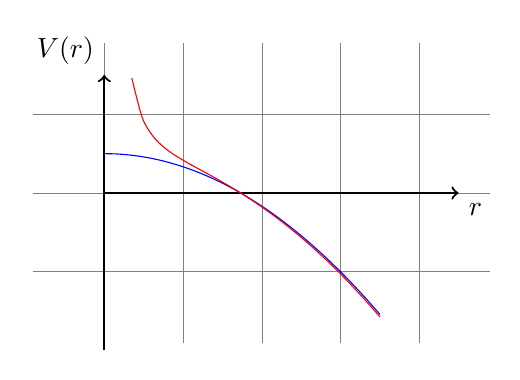
\begin{tikzpicture}
\draw[step=1cm,gray,very thin] (-0.9,-1.9) grid (4.9,1.9);
\draw[thick,->] (0,0) -- (4.5,0) node[anchor=north west] {$r$};
\draw[thick,->] (0,-2.0) -- (0,1.5) node[anchor=south east] {$V(r)$};

\draw[scale=0.5, domain=0:7, smooth, variable=\x, blue] plot ({\x}, {1-\x*\x/12});
\draw[scale=0.5, domain=0.7:7, smooth, variable=\x, red] plot ({\x}, {1-1*(1/12-1/(\x*\x))-\x*\x/12});

\end{tikzpicture}
\end{center}
3.) Small radial velocity means $E\approx1$ and $L=0$
\begin{align}
\dot{r}&=\sqrt{E^2-1+\frac{r^2}{R^2}}\\
&=\sqrt{E^2-1}\sqrt{1+\frac{r^2}{R^2(E^2-1)}}\\
\frac{\dot{r}}{\sqrt{E^2-1}}&=\sqrt{1+\frac{r^2}{R^2(E^2-1)}}\\
\dot{y}&=\sqrt{1+\frac{y^2}{R^2}}\qquad(y=r/\sqrt{E^2-1})
\end{align}
Now set $\lambda=\tau/R$ then
\begin{align}
\frac{\partial y}{\partial \lambda}=\frac{\partial y}{\partial \tau}\frac{\partial \tau}{\partial \lambda}=\frac{1}{R}\frac{\partial y}{\partial \tau}
\end{align}
and with $z=y/R$
\begin{align}
\frac{\dot{y}}{R}&=\sqrt{1+\frac{y^2}{R^2}}\\
z'&=\sqrt{1+z^2}
\end{align}
with the solutions $z=\sinh(\lambda+c)$ and resubstitution we obtain
\begin{align}
r(\lambda)=R\sqrt{E^2-1}\sinh\lambda/R
\end{align}
and
\begin{align}
\Delta\lambda=R\cdot\text{arcsinh}\frac{1}{\sqrt{E^2-1}}
\end{align}
\textcolor{red}{
\begin{align}
\frac{dr}{d\lambda}&=\sqrt{E^2-1}\cosh\lambda/R\\
&=\sqrt{E^2-1}\sqrt{1+\sinh^2\lambda/R}\\
&=\sqrt{E^2-1}\sqrt{1+\frac{r^2}{R^2\sqrt{E^2-1}}}\\
&\rightarrow t=\int_0^R\frac{dt}{d\lambda} d\lambda=\int dr\frac{-E}{1-\frac{r^2}{R^2}}\frac{1}{\sqrt{E^2-1+\frac{r^2\sqrt{E^2-1}}{R^2}}}
\end{align}
}

\subsection{Problem 2.5 - Distances}
Metric distance $d_M$, luminosity distance $d_L$ 
\begin{align}
d_M   &=S_k(\chi)\\
d_L(z)&=(1+z)d_M(z)\\
d_A(z)&=\frac{d_M(z)}{1+z}
\end{align}

\subsection{Problem 2.6 - Friedmann universes}
\subsection{Problem 2.7 - Einsteins biggest blunder}
\subsection{Problem 2.8 - The accelerating universe}
\subsection{Problem 2.9 - Phantom Dark energy}

\subsection{Exercise 3.1}
Let's first rewrite the Zeta function as an integral starting with the common definitions
\begin{align}
    \Gamma(s)&=\int_0^\infty t^{s-1}e^{-t} dt\\
    \zeta(s)&=\sum_{n=1}^\infty\frac{1}{n^s}
\end{align}
Then with $t/n=x$ and $dx=dt/n$
\begin{align}
	\zeta(s)\Gamma(s)
	&=\sum_{n=1}^\infty\int_0^\infty \frac{1}{n^s}t^{s-1}e^{-t} dt\\
	&=\sum_{n=1}^\infty\int_0^\infty \frac{1}{n^s}t^{s-1}e^{-t} n\,dx\\
	&=\sum_{n=1}^\infty\int_0^\infty \frac{t^{s-1}}{n^{s-1}}e^{-nx} dx\\
	&=\int_0^\infty x^{s-1}\sum_{n=1}^\infty e^{-nx} dx\\
	&=\int_0^\infty \frac{x^{s-1}}{e^{x}-1} dx
\end{align}
we obtain
\begin{align}
\zeta(s)&=\frac{1}{\Gamma(s)}\int_0^\infty \frac{x^{s-1}}{e^{x}-1} dx.
\end{align}
Now
\begin{align}
J_{-}(0)&=\int_0^\infty\frac{\xi^3}{e^\xi-1}d\xi\\
&=\Gamma(4)\zeta(4)\\
&=3!\zeta(4)
\end{align}
Furthermore we can write
\begin{align}
J_{-}(0)
&=\int_0^\infty\frac{\xi^3}{e^\xi-1}d\xi\\
&=\int_0^\infty\frac{\xi^3}{(e^{\xi/2}-1)(e^{\xi/2}+1)}d\xi\\
&=\frac{1}{2}\int_0^\infty\frac{\xi^3}{e^{\xi/2}-1}d\xi-\frac{1}{2}\int_0^\infty\frac{\xi^3}{e^{\xi/2}+1}d\xi\\
&=8\int_0^\infty\frac{x^3}{e^{x}-1}dx-8\int_0^\infty\frac{x^3}{e^{x}+1}dx\\
&=8J_{-}(0)-8J_{+}(0)\\
&\rightarrow J_{+}=\frac{7}{8}J_{-}(0)
\end{align}



\newpage
\section{{\sc Dodelson, Schmidt} - Cosmology (2nd edition)}
\subsection{1.2}
We start with 
\begin{align}
\rho_\text{cr}&=\frac{3H_0^2}{8\pi G}\\
H(t)&=\frac{1}{a}\frac{da}{dt}\\
H(t)^2
&=\frac{8\pi G}{3}\left[\varrho(t)+\frac{\Lambda}{3}-\frac{k}{a^2}\right]\\
&=\frac{8\pi G}{3}\left[\rho(t)+\frac{\rho_\text{cr}-\rho(t_0)}{a^2}\right]\\
&=\frac{8\pi G}{3}\left[\Omega_m\left(\frac{a_0}{a}\right)^3\rho_\text{cr}+\Omega_\Lambda\rho_\text{cr}+\frac{\rho_\text{cr}-\rho(t_0)}{a^2}\right]\\
&=H_0^2\left[\Omega_m\left(\frac{a_0}{a}\right)^3+\Omega_\Lambda+\frac{\rho_\text{cr}-\rho(t_0)}{\rho_\text{cr}a^2}\right]\\
\end{align}
and assume $\rho_\text{cr}=\rho(t_0)$ (same as Euclidean $k=0$?!?) and $\Omega_\Lambda+\Omega_m=1$ and $a_0=1$
\begin{align}
dt&=\frac{da}{a}\frac{1}{H(t)}\\
&=\frac{da}{a}\frac{1}{H_0\sqrt{\Omega_m\left(\frac{a_0}{a}\right)^3+\Omega_\Lambda}}\\
&=\frac{1}{H_0}\frac{da}{a}\left[\frac{1-\Omega_\Lambda}{a^3}+\Omega_\Lambda\right]^{-1/2}
\end{align}
(a) Now with $\Omega_\Lambda=0$
\begin{align}
dt&=\frac{1}{H_0}\frac{da}{a}a^{3/2}=\frac{1}{H_0}da\;a^{1/2}\\
&\rightarrow t-t_i=\frac{2}{3H_0}(a^{3/2}-a_i^{3/2})\\
&\rightarrow a(t)=\left(\frac{3H_0}{2}(t-t_i)+a_i^{3/2}\right)^{2/3}
\end{align}
with $a(t=0)=0$
\begin{align}
a(t)&=\left(\frac{3H_0}{2}t\right)^{2/3}\\
&\rightarrow T=\frac{2}{3H_0}
\end{align}
(b) ...

\subsection{1.3 Lyman-$\alpha$ splitting in hydrogen isotopes}
The energy eigenvalues are
\begin{align}
E_n
&=-\frac{1}{2}\mu c^2\frac{\alpha^2}{n^2}\\
&=-\frac{1}{2}\frac{m_eM_\text{nuc}}{m_e+M_\text{nuc}} c^2\frac{\alpha^2}{n^2}
\end{align}
then
\begin{align}
\Delta E_{2\rightarrow1}
&=-\frac{1}{2}\frac{m_eM_\text{nuc}}{m_e+M_\text{nuc}} c^2\alpha^2\left(\frac{1}{2^2}-\frac{1}{1^2}\right)\\
&=\frac{3}{8}\frac{m_eM_\text{nuc}}{m_e+M_\text{nuc}} c^2\alpha^2\\
&=\frac{3}{8}\frac{m_eM_\text{nuc}}{M_\text{nuc}(1+m_e/M_\text{nuc})} c^2\alpha^2\\
&=\frac{3}{8}\frac{m_e}{1+m_e/M_\text{nuc}} c^2\alpha^2
\end{align}
and
\begin{align}
\Delta E^\text{D}_{2\rightarrow1}
&=\frac{3}{8}\frac{m_e}{1+m_e/2m_p} c^2\alpha^2\\
\Delta E^\text{H}_{2\rightarrow1}
&=\frac{3}{8}\frac{m_e}{1+m_e/m_p} c^2\alpha^2\\
\rightarrow \Delta E^\text{D}_{2\rightarrow1}&= \Delta E^\text{H}_{2\rightarrow1}\frac{1+m_e/m_p}{1+m_e/2m_p}
\end{align}
and with $E=hc/\lambda$
\begin{align}
\lambda^\text{D}_{2\rightarrow1}&=\frac{hc}{\Delta E^\text{D}_{2\rightarrow1}}\\
&=\frac{hc}{\Delta E^\text{H}_{2\rightarrow1}}\frac{1+m_e/2m_p}{1+m_e/m_p}\\
&=\lambda^\text{H}_{2\rightarrow1}\frac{1+m_e/2m_p}{1+m_e/m_p}\\
&=\lambda^\text{H}_{2\rightarrow1}\left(1+\frac{m_e}{2m_p}\right)\left(1-\frac{m_e}{m_p}\right)\\
&\simeq\lambda^\text{H}_{2\rightarrow1}\left(1-\frac{1}{2}\frac{m_e}{m_p}\right)\\
&=1215.67\text{\AA}
\end{align}
furthermore
\begin{align}
c\frac{\Delta\lambda}{\lambda}&=
c\frac{\lambda^\text{D}_{2\rightarrow1}-\lambda^\text{H}_{2\rightarrow1}}{\lambda^\text{H}_{2\rightarrow1}}\\
&=\left(1-\frac{1}{2}\frac{m_e}{m_p}\right)\\
&=0.999727c
\end{align}

\subsection{1.4 Planck law for CMB}
Insider hint $1\text{MJy} =10^6\text{Jansky}=10^6\cdot10^{-26}\text{J}\cdot\text{s}^{-1}\cdot\text{Hz}^{-1}\cdot\text{m}^{-2}$. We start with $c=\lambda\nu=2\pi\nu/k$
\begin{align}
I_\nu=\frac{4\pi\hbar\nu^3}{c^2}\frac{1}{e^{2\pi\hbar\nu/k_\text{B}T}-1}
\end{align}
which has the unit energy per area (per frequency per time are cancelling)
\begin{align}
\frac{\text{Js}\cdot \text{s}^{-3}}{\text{m}^2/\text{s}^2}=\text{J}\cdot\text{m}^{-2}
\end{align}
then
\begin{align}
\frac{I_\nu d\nu}{d\Omega}
\end{align}

\section{{\sc Mukhanov} - Physical foundations of cosmology, 2005}


\end{document}